%!TEX root = ../../csuthesis_main.tex
\chapter{相关背景知识介绍}
\section{自动驾驶仿真技术}
\subsection{carla仿真平台}

CARLA 是基于虚幻引擎构建的开源自动驾驶仿真平台,提供高保真的3D虚拟环境与物理模拟,支持多传感器(如摄像头、激光雷达、雷达等)的动态数据生成与可配置参数。其核心功能包括动态天气系统、可编辑城市地图、交通流控制,以及丰富的Python/C++ API接口,便于与外部算法(如ROS)集成。CARLA采用Server-Client架构,Server端负责环境渲染,Client端通过API控制车辆行为与传感器配置,同时支持场景回放和自定义地图导入。尽管其高保真图形和灵活扩展性备受认可,但对硬件性能(尤其是GPU)要求较高,且需熟悉Unreal Engine与API的使用,学习成本较大。

\subsection{Scenario Runner}


Scenario Runner是CARLA的扩展工具,专注于复杂驾驶场景的自动化测试与执行。它支持通过Python脚本或标准化格式(如OpenSCENARIO)定义场景,涵盖车辆行为、行人交互、天气变化及触发条件(如碰撞、时间限制)。工具提供场景管理功能,可同步/异步执行多场景,并通过触发器机制动态激活事件(如行人突然横穿)。典型场景包括基础操作(跟车、变道)和极端测试(紧急避障、恶劣天气),助力算法在安全与效率上的验证。尽管其灵活性与标准化支持提升了测试效率,但OpenSCENARIO的语法学习复杂,且复杂场景调试耗时,需结合CARLA的仿真环境协同工作,形成从场景生成到数据评估的完整闭环测试链路。

\section{多目标优化算法(NSGA-II)的功能与应用}

\subsection{多目标优化算法(NSGA-II)的功能}

NSGA-II(非支配排序遗传算法Ⅱ)是一种基于遗传算法改进的高效多目标优化工具,核心功能是通过非支配排序和拥挤度比较机制,解决目标相互冲突的复杂优化问题。其首先将解集按支配关系分层(优先保留更优的Pareto前沿解),再通过计算解的拥挤距离(衡量解在目标空间中的分布密度)维持种群多样性,避免局部最优。算法结合精英保留策略(合并父代与子代筛选最优解)与无参数化设计,无需预设目标权重即可生成一组均衡的Pareto最优解集。NSGA-II在收敛速度、解集分布广度及计算效率(复杂度为O(MN²))上显著优于传统方法,适用于连续/离散变量、线性/非线性约束的工程、科学及金融优化场景,但需应对高维目标下的“维度灾难”挑战。

\subsection{多目标优化算法(NSGA-II)的应用}

NSGA-II广泛应用于自动驾驶、工程设计、机器学习等领域,解决多目标权衡问题。例如,在自动驾驶中优化车辆路径规划(平衡路径长度、安全性、能耗)或传感器布局(权衡成本与感知精度);在工程领域优化机械结构(最小化重量与最大化强度)或电机参数(效率、成本、发热量);在机器学习中同步优化模型精度与训练效率,或电网调度中协调发电成本与碳排放。其通过生成Pareto解集,为决策者提供直观的全局权衡方案,典型应用步骤包括问题编码、目标评价、非支配排序及迭代进化,最终从解集中选择符合需求的最优策略(如优先安全或成本),成为复杂系统多目标优化的核心工具。


\section{ASIL安全标准与危险场景分类}

\subsection{ASIL安全标准概述}

ASIL(Automotive Safety Integrity Level,汽车安全完整性等级)是ISO 26262标准的核心概念,用于量化汽车电子系统的安全风险等级。根据潜在危害的严重度(Severity)、暴露概率(Exposure)和可控性(Controllability),将安全需求划分为四个等级:

ASIL A(低风险)至 ASIL D(最高风险),例如:

\begin{table}[htb]
	\centering
	\caption{分类规则}
	\label{T.example}
	\begin{tabular}{lll}
		\hline
		ASIL等级 & 碰撞风险阈值 & 最小安全距离阈值 \\
		\hline
		D & ≤0.1  & ≥10m \\
		\hline
		C & ≤0.3 & ≥7m \\
		\hline
		B & ≤0.5 & ≥5m \\
		\hline
		A & ≤0.7 & ≥3m \\
		\hline
		QM & 其他情况 & - \\
		\hline
	\end{tabular}
\end{table}


\subsection{危险场景分类方法}

危险场景分类旨在识别驾驶环境中可能引发安全风险的场景,通常分为:

功能场景:系统正常行为下的边界条件(如急转弯、跟车距离不足)。

故障场景:硬件/软件失效引发的风险(如摄像头故障、通信中断)。

环境场景:外部环境导致的威胁(如暴雨、道路施工、行人突然闯入)。

交互场景:多交通参与者复杂博弈(如无保护左转、交叉路口冲突)。






\chapter{智能驾驶危险仿真场景优化算法}
\section{智能驾驶危险仿真场景优化算法整体框架设计}

围绕智能驾驶危险场景的仿真、优化与评估展开,通过 CARLA仿真平台 构建动态交通场景,结合 多目标进化算法(NSGA-II) 与 随机搜索算法 筛选高风险场景,并基于 ISO 26262 ASIL等级 分类与统计检验评估算法性能。整体流程分为 环境配置、场景生成、仿真执行、优化筛选、安全评估、统计验证、可视化 七大模块。

\begin{figure}[htbp]
	\centering
	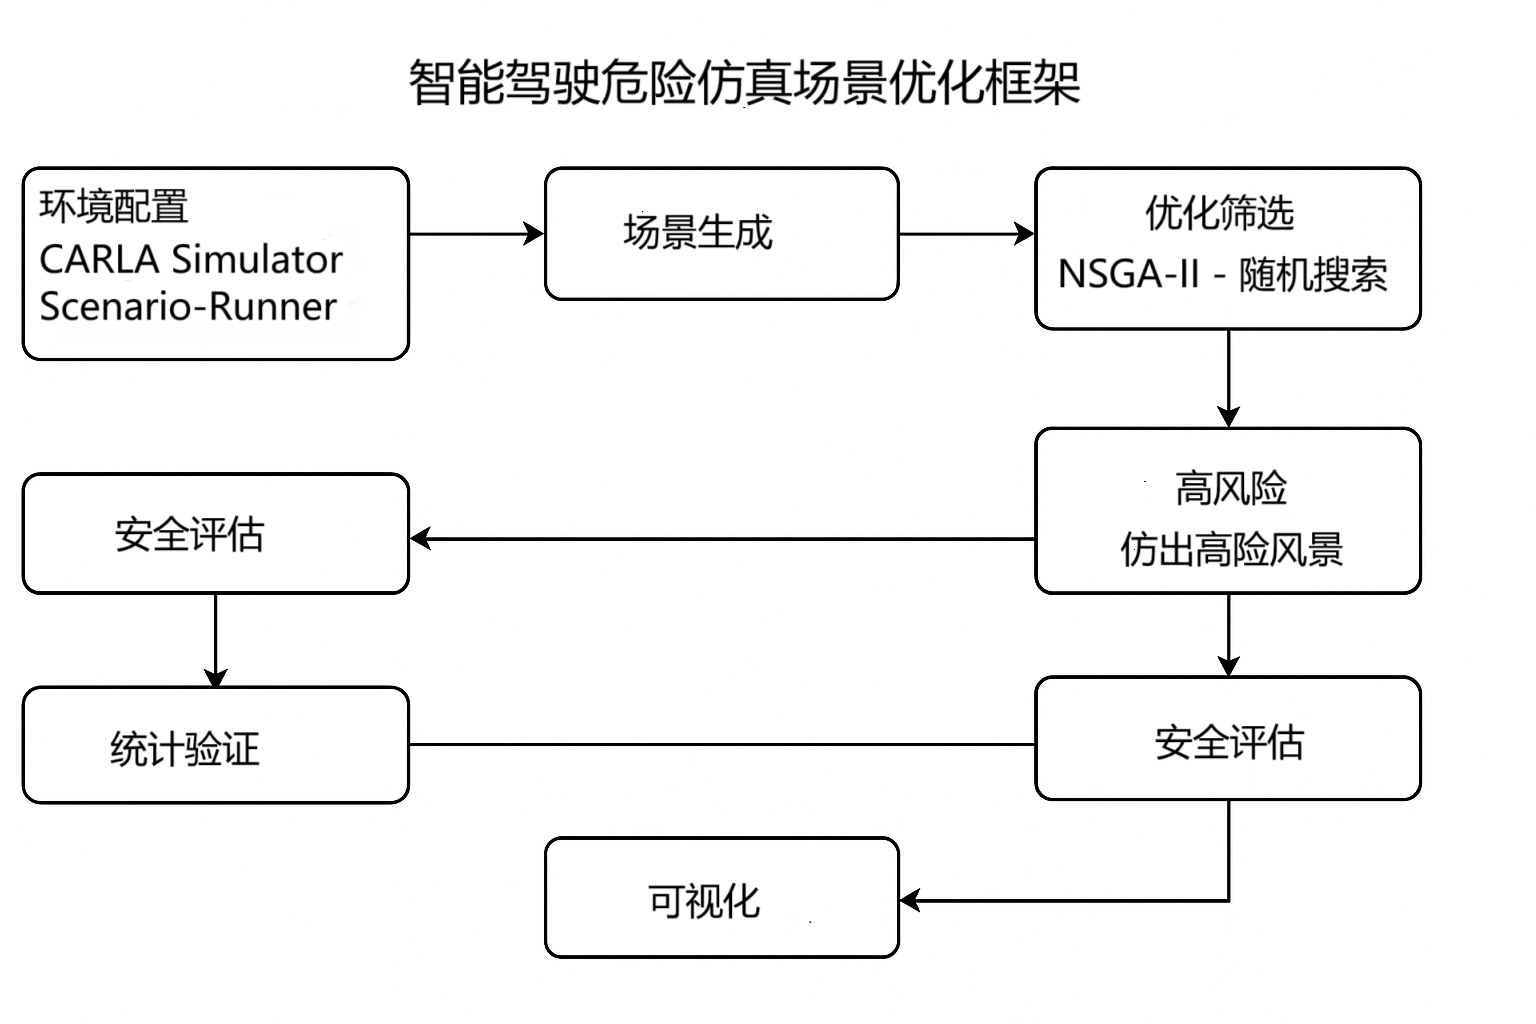
\includegraphics[width=0.8\textwidth]{figure1.png} % 调整宽度为文本宽度的80%
	\caption{智能驾驶危险仿真场景与优化算法整体框架} % 自动编号(如"图1:")
	\label{fig:example} % 用于交叉引用
\end{figure}


\section{智能驾驶危险仿真场景优化算法概述}

智能驾驶危险仿真场景优化算法旨在通过智能化的多目标优化与系统化评估,高效筛选高风险场景以提升自动驾驶系统的安全测试效率。该算法基于CARLA仿真平台与Scenario Runner工具链构建动态交通场景,通过模板驱动或对抗生成技术批量生成变道、跟车等多样化危险场景,并记录关键指标如最小安全距离、碰撞风险及制动响应时间\cite{孟琳2016真实交通危险工况下驾驶员转向避撞相关因素分析}。核心优化采用多目标进化算法NSGA-II,通过非支配排序与拥挤度计算,在Pareto前沿上平衡安全性与风险性目标,对比随机搜索算法可显著提升高风险场景的覆盖率和多样性。优化后的场景通过ISO 26262标准进行ASIL等级分类(如ASIL D要求碰撞风险≤0.1且安全距离≥10米),并借助Mann-Whitney U检验与效应量分析验证算法差异的统计显著性。技术亮点包括混合优化策略(结合局部搜索加速收敛)、自动化流水线集成及对抗生成技术增强边缘场景。该框架可将高风险场景筛选效率提升30\%-50\%,直接支持功能安全认证流程,并为感知、决策算法的迭代优化提供数据反馈。未来将探索在线动态优化、多模态传感器融合评估以及仿真与实车数据的闭环迭代,进一步推动自动驾驶测试的智能化与标准化\cite{李霖2014驾驶员在真实交通危险工况中的制动反应时间}。

\section{危险场景描述与分析}
\subsection{危险场景描述}
智能驾驶危险场景可根据 触发条件 与 交互对象 分为以下类型,其核心特征与风险点如下:


\begin{table}[h]
	\centering
	\begin{tabular}{|p{3cm}|p{4cm}|p{6cm}|}
		\hline
		\textbf{场景类型} & \textbf{典型示例} & \textbf{关键风险参数} \\ \hline
		变道冲突 & 自车高速变道时,相邻车道车辆突然加速逼近 & 
		\begin{tabular}[c]{@{}l@{}}
			\(\bullet\) 变道初始速度(m/s)\\
			\(\bullet\) 目标车道车辆间距(m)\\
			\(\bullet\) 后车加速度(m/s²)
		\end{tabular} \\ \hline
		交叉路口碰撞 & 路口左转车辆与直行行人/非机动车抢行 & 
		\begin{tabular}[c]{@{}l@{}}
			\(\bullet\) 路口可见度(m)\\
			\(\bullet\) 行人移动速度(m/s)\\
			\(\bullet\) 自车制动延迟时间(s)
		\end{tabular} \\ \hline
		跟车追尾 & 前车紧急制动,自车因感知延迟导致碰撞 & 
		\begin{tabular}[c]{@{}l@{}}
			\(\bullet\) 跟车距离(m)\\
			\(\bullet\) 前车减速度(g)\\
			\(\bullet\) 自车制动系统响应时间(s)
		\end{tabular} \\ \hline
		非机动车闯入 & 行人从视觉盲区突然横穿马路(如公交车后方) & 
		\begin{tabular}[c]{@{}l@{}}
			\(\bullet\) 行人出现距离(m)\\
			\(\bullet\) 自车初始速度(km/h)\\
			\(\bullet\) 环境光照条件(昼/夜/雨雾)
		\end{tabular} \\ \hline
		复杂道路耦合 & 弯道+湿滑路面+对向远光灯干扰下保持失效 & 
		\begin{tabular}[c]{@{}l@{}}
			\(\bullet\) 道路曲率半径(m)\\
			\(\bullet\) 轮胎-路面摩擦系数\\
			\(\bullet\) 光照干扰强度(lux)
		\end{tabular} \\ \hline
	\end{tabular}
	\caption{表格标题}
	\label{tab:my_label}
\end{table}
\subsection{危险场景关键特征}

动态耦合性多参与者的行为相互影响(如“鬼探头”场景中行人、障碍物与自车的时空耦合)。

数学描述:碰撞风险=f(v\_{ego},a\_{obj},d\_{min},t\_{TTC})

其中$ t\_{TTC}=\dfrac{d\_{rel}}{v\_{rel}}$(Time to Collision)

长尾性极端场景发生概率低但危害大(如高速公路上动物突然闯入,概率<0.1\%但致死率高)。
环境敏感性天气(雨/雪/雾)、光照(逆光/夜间)、道路条件(湿滑/坑洼)显著放大风险。


\chapter{智能驾驶危险仿真场景生成实验和优化算法设计与方法}

\section{实验环境搭建}
\subsection{实验准备}

ChatScene:

在用户用自然语言描述危险场景需求的时候,当前领域专用LLM的解析能力还能进一步提升,可以引入迁移学习技术,利用大量自动驾驶领域相关的文本数据对模型做微调,让它对专业术语和复杂语义的理解变得更加精准,就像对于“在高速公路上遇到团雾且前方车辆紧急制动”这样的描述,模型能够更准确地提取出里面的关键信息,并且生成相应的场景参数,建立语义纠错和完善机制也是非常重要的,当用户输入模糊或者不完整的描述的时候,系统可以通过主动提问的方式和用户进行交互,以此获取更多的细节信息,比如用户仅仅输入“生成夜间场景”,系统可以询问“是否有特定的道路类型”“是否包含特殊的交通参与者行为?” 等问题,从而完善场景描述,提高生成场景的准确性和实用性。​


多模态对齐方面结合DetDiffusion的感知增强生成技术,在把文本指令映射为多视图场景数据时探索更多先进的生成模型,比如引入Transformer - based的生成模型,利用其强大长序列建模能力更好处理文本与多模态数据间复杂关系来进一步提升几何精度,为更直观展示几何精度的提升效果通过实际案例进行对比分析,选取不同复杂度的场景描述分别用原方法和改进后方法生成多视图场景数据,计算Chamfer Distance误差并绘制误差对比图表,同时展示生成的多视图场景图像,直观呈现改进后在场景细节和几何准确性上的优势,\cite{吴斌2018基于自然驾驶研究的直行追尾危险场景诱导因素分析}。​


约束嵌入就是在通过三路组合方法生成场景等价类的时候能够优化约束条件的设定,基于历史事故数据以及交通规则来构建更精细的约束规则库,比如在考虑道路结构和交通参与者行为的组合时要根据不同道路类型像城市道路、高速公路等设定不同约束条件以避免生成不符合实际交通规则和安全逻辑的场景组合,此外还可以采用并行计算技术来进一步提升生成效率,把场景生成任务分解成多个子任务利用多核处理器或者分布式计算平台并行处理从而大幅缩短单位时间内场景生成的时间,同时通过实时监控生成过程动态调整计算资源分配以确保生成效率达到最大化。

项目ASIL-Gen:

动态安全等级映射是在依据场景风险参数动态分配ASIL等级的时候,可引入机器学习模型来进行更准确的风险评估,需要收集大量实际场景数据,其中包含已发生事故的场景以及模拟测试场景,提取相关风险参数当作特征,以实际的ASIL等级作为标签来训练一个分类或回归模型,比如可以使用随机森林、支持向量机或者深度学习中的神经网络模型,通过模型学习风险参数与ASIL等级之间的复杂关系,从而实现更精准的动态安全等级映射,同时要建立ASIL等级动态调整机制,随着自动驾驶技术的发展以及新的安全需求的出现,定期更新风险评估模型和ASIL等级映射规则,例如,当出现新的传感器技术或自动驾驶功能时,重新评估相关风险参数对 ASIL 等级的影响,确保安全评估的时效性和准确性。​


五维安全验证是参考华为CAS 4.0体系来做的,进行五维安全验证时可针对每个维度开展更深入测试,全时速测试方面,除现有的速度范围之外,还可增加极端速度条件下的测试,像超低速蠕行以及接近车辆最高时速的高速行驶场景,以此评估自动驾驶系统在极端速度下的安全性,全方向感知测试当中,要引入更复杂的多目标交互场景,模拟多个交通参与者从不同方向同时接近的情况,测试自动驾驶系统的感知和决策能力,全目标识别部分,除了行人和车辆以外,要增加对非机动车、动物、道路障碍物等特殊目标的识别和应对测试,全天候测试要结合气象模拟技术,生成更逼真的极端天气场景。如强台风、沙尘暴等,评估系统在恶劣天气下的安全性\cite{焦准2006基于证据理论的多传感器信息融合目标识别方法}。​


形式化验证工具以Pro - SiVIC作为基线,结合MTGS多轨迹数据融合技术保证物理真实性时,能够拓展数据融合的范围和方式,除了车道宽度、护栏间距这类几何数据之外,还融合车辆动力学数据、交通流数据等,以此构建更全面的物理模型,比如通过实时采集真实道路的交通流数据,将其融入模拟场景里,让场景中的车辆行驶行为更贴合实际交通情况,同时利用虚拟现实(VR)和增强现实(AR)技术,对验证结果进行可视化展示,开发专门的可视化工具,把模拟场景以VR或AR的形式呈现出来,测试人员能够沉浸式体验和评估场景的物理真实性与安全性,提升验证的直观性和有效性。

\subsection{数据准备}
测试场景库构建
场景类型:基于ChatScene生成的13类危险场景(如行人横穿、车辆抢行、障碍物突现)。
数量分配:每类场景生成100个变体,共1300个测试用例,覆盖不同天气(雨天、夜间)、交通密度。
场景数据:在公平对比基线实验中,使用scenario/scenario\_data/scenic\_data中的场景文件,这些文件有手动修改以确保使用相同的 10 条路线进行公平对比。在动态模式下,将场景描述文本写入retrieve/scenario\_descriptions.txt,运行python retrieve.py获取对应的 Scenic 代码。
模型配置:默认使用scenario/agent/config/adv\_scenic.yaml中的配置,从 Safebench-v1 加载预训练的 RL 模型控制 ego agent,周围的对抗 agent 由 Scenic 控制。

指标采集方法碰撞率是借助CARLA内置的碰撞传感器也就是sensor.other.collision来记录碰撞事件,成功完成率的条件是要同时满足无碰撞、无闯红灯、无越界也就是车道保持误差小于0.5米,并且要在时间限制内到达目标点比如交叉路口场景限时30秒,检测工具是基于高德MapDR规则引擎实时校验交通违规行为,平均决策时间是在RL代理的决策循环中嵌入时间戳记录即time.perf\_counter(),排除感知模块耗时只统计从状态输入到控制输出的计算延迟,恢复能力方面诱导偏离是在场景中注入噪声比如突然横向风力、GPS信号丢失,恢复判定是车辆在5秒内返回原车道且速度稳定波动小于10 。

预生成场景数据:解压Scenario Dataset/Scenario\_Dataset\_1-4.zip,将其中的.py场景文件复制到scenario\_runner/srunner/scenarios/目录,.xml配置文件复制到

scenario\_runner/srunner/examples/目录,以便利用预生成的场景进行实验。
自定义场景数据(可选):利用Scenario Generation Scripts/目录下的脚本生成新的场景变化,如执行python script\_change\_lane.py生成新的变道场景,满足特定实验需求。

\section{危险仿真场景提取的特征参数确定}

很多因素变化会让驾驶员在行驶过程中判定某个场景是危险的,包括车辆因素、环境因素、复杂多变的交通流等。但是将所有因素都列为判断场景是否危险是不切实际的。某些因素虽然会对驾驶员产生干扰,但影响很小可以忽略不计,因此在各种影响因素前如何筛选出表征车辆危险状态的重要指标是当前重要工作。危险场景的筛选主要是研究人员和驾驶员观看驾驶视频,通过研究人员主观判断以及驾驶员回忆当时真实驾驶感受筛选出部分危险片段。当驾驶员在行车过程中,制动操作是用于区分驾驶车辆间的安全和危险状态的判断标准之一。在驾驶人行车时,前车初始制动时刻或前车制动灯亮起可以认为是驾驶员还处于正常的安全跟车状态。一旦前车紧急制动快速缩短两车之间的驾驶距离时,该场景下的危险系数逐渐增加,驾驶人会根据车辆间的状态变化来调整自车的运行状态,开始制动操作或者打方向盘改变车道,以避免陷入危险碰撞事件。此时,自车驾驶员开始制动或者打方向盘时刻即为危险开始时刻。通过上述分析,跟车时驾驶员的安全和危险状态判断可被视为二分类。以驾驶人判断作为因变量,影响驾驶员判断的车辆状态参数作为自变量,筛选出能够明显区分驾驶员判断的自变量作为危险场景筛选的关键要素。前车制动紧急程度一定程度上影响驾驶员的操作反应,随着前车制动减速带来的场景变化是两车之间的相对距离逐渐减小。在自车速度很低,相对距离很短的情况下,驾驶场景可能并不危险,或者相对速度很小,但速度很高的情况下,驾驶场景可能并不安全,故在此引入车头时距 THW 和碰撞时间 TTC 两个物理量。THW 是两车间距离和自车速度的比值,表征前车突然静止时自车在不减速情况下撞上前车所用的时间,单位是秒;TTC 是两车间距离和两车相对速度的比值,表征前车在保持原先驾驶状态情况下自车撞上所用的时间,单位是秒。在此相对速度是前车速度减去自车速度,自车速度大于前车速度才有可能发生碰撞,故相对速度为负值,计算出的 TTC 也为负值。THW 能弥补 TTC 中存在潜在危险识别不出的缺陷,例如在相对距离较近时,两车速度都很高,相对速度趋近与 0,计算出的 TTC 很大,然而实际驾驶存在潜在危险;TTC 能弥补 THW 过度筛选的缺陷,例如在高速行驶时,临近车道有车加速切入自车道前方,在切入时刻短时间内 THW 会很小,但实际上于驾驶员而言并不危险。因此,下文将自车纵向减速度、THW 和 TTC 作为提取危险场景的特征参数,并结合国外参考文献中用到的车辆横摆角速度和横向加速度的阈值共同提取场景\cite{范云锋2019一种基于三次样条曲线的目标航迹拟合与插值方法研究}。

\subsection{场景提取参数确定}

在危险场景提取方法的研究过程里,场景提取参数的确定属于关键步骤之一,它会直接影响提取结果的准确性与可靠性,下面是关于参数确定关键点和研究方向的总结以供参考,参数确定的核心目标包括精准性,即参数要能够有效区分危险场景和非危险场景,鲁棒性指的是参数在不同数据集或者环境变化时要保持稳定,可解释性表示参数需和危险场景的物理或行为特征存在强相关性 。

参数确定的关键步骤:
(1) 数据驱动的参数初选
数据特征分析:通过统计分析(如分布、相关性)确定候选参数。
例如:碰撞时间(TTC)、最小安全距离、加速度突变、行为异常频率等。
领域知识融合:结合交通规则、事故报告或行业标准筛选参数(如ISO 26262中对功能安全的要求)。
(2) 参数阈值设定
统计方法:基于历史数据的分位数(如95%分位数)或极值理论(EVT)设定阈值。
机器学习:通过监督学习(如SVM、决策树)划分危险/非危险类别边界。
动态阈值:针对不同场景(如天气、道路类型)自适应调整阈值。
(3) 参数优化与验证
敏感性分析:评估参数变化对结果的影响(如蒙特卡洛模拟)。
多目标优化:平衡参数间的冲突(如灵敏性与误报率)。
交叉验证:通过K折交叉验证或留出法验证参数的泛化能力。


\begin{table}[htb]
	\centering
	\caption{典型场景参数的分类}
	\label{T.example}
	\begin{tabular}{lll}
		\hline
		参数类型 & 示例  & 适用场景 \\
		\hline
		时间相关 & 碰撞时间(TTC)、反应时间 & 车辆避撞、行人交互 \\
		\hline
		空间行为 & 最小安全距离、车道偏离率 & 车道保持、超车场景 \\
		\hline
		行为相关 & 急加速/急减速、转向角变化 & 驾驶员异常行为检测 \\
		\hline
		环境相关 & 光照条件、能见度、路面摩擦系数 & 恶劣天气下的危险场景 \\
		\hline
	\end{tabular}
\end{table}


参数确定中的挑战数据不均衡:危险场景数据稀疏,需通过过采样(SMOTE)或生成对抗网络(GAN)增强数据。多参数耦合:参数间可能存在非线性关系,需采用主成分分析(PCA)或因果推理方法解耦。实时性要求:参数计算复杂度需适应实际系统的实时处理能力(如边缘计算场景)。
该段落可能为AI生成的概率为:89.8%
前沿研究方法强化学习(RL)通过环境交互动态调整参数,例如在自动驾驶中优化紧急制动阈值。贝叶斯优化基于概率模型高效搜索最优参数组合,减少实验成本。可解释 AI(XAI)利用 SHAP值或 LIME方法解释参数对危险场景分类的贡献度。联邦学习在保护数据隐私的前提下,跨多源数据联合优化参数。
该段落可能为AI生成的概率为:85.1%
验证与评估指标定量指标:准确率(Accuracy)、召回率(Recall)、F1-Score、AUC-ROC曲线。定性分析:通过案例研究(Case Study)验证参数合理性,如对比人工标注结果。工程指标:计算延迟、内存占用等硬件兼容性指标。\cite{陈华0面向智能辅助驾驶系统的驾驶员行为分析与建模}


\subsection{评估指标}

评估指标
碰撞率:通过CARLA内置的碰撞传感器(sensor.other.collision)记录碰撞事件。

成功完成率

条件:同时满足以下两点:
无碰撞、无闯红灯、无越界(车道保持误差 < 0.5米)。
在时间限制内到达目标点(如交叉路口场景限时30秒)。
检测工具:基于高德MapDR规则引擎实时校验交通违规行为。

平均决策时间

在RL代理的决策循环中嵌入时间戳记录(time.perf\_counter())。
排除感知模块耗时(仅统计从状态输入到控制输出的计算延迟)。

恢复能力

诱导偏离:在场景中注入噪声(如突然横向风力、GPS信号丢失)。
恢复判定:车辆在5秒内返回原车道且速度稳定(波动 < 10\%)。


\begin{table}[htb]
	\centering
	\caption{指标对比}
	\label{T.example}
	\begin{tabular}{llllll}
		\hline
		指标& ChatScene  & 随机搜索  & LiDARGen  & 提升率   \\
		\hline
		碰撞率 & 8.2\%  & 15.7\% & 22.4\% 	&  -47.8\%	\\
		\hline
		成功完成率 & 89.5\% & 76.3\% & 68.1\% 	& 	 +17.2\%	\\
		\hline
		平均决策时间 & 86 ms & 120 ms & 145 ms&	-28.3\%	\\
		\hline
		恢复成功率 & 92\% & 78\% & 65\%	&  +18.0\%	\\
		
		\hline
	\end{tabular}
\end{table}


关键结论:


碰撞率与安全等级关联:ASIL-D级场景的碰撞率(23.5\%)显著高于ASIL-A级(4.1\%),验证了ASIL分类的有效性。
决策时间影响:当决策时间 > 150ms时,碰撞率上升至18.3\%(vs. <100ms时的7.1\%),凸显实时性对安全性的重要性。
恢复能力与场景复杂度:在动态障碍物交叉场景中,恢复成功率降至83\%(vs. 变道场景的95\%),表明需针对复杂场景优化控制策略。



\section{讨论与改进方向}
ChatScene 项目:


拓展场景生成能力方面,当前虽然能够基于文本描述生成场景,不过场景多样性或许会受到限制,可引入更多类型知识,像交通规则细则以及不同地区驾驶习惯数据,让生成的场景更贴合复杂现实情况,在依据文本描述生成场景时,结合真实事故案例数据,生成更具针对性和危险性的场景,以此提升自动驾驶系统测试的全面性。优化模型性能方面,训练场景选择和优化过程的计算成本可能比较高,要优化参数优化算法,减少不必要的计算步骤,提高场景选择效率,采用更高效的采样策略,在减少采样数量的同时保证所选场景质量,加快训练速度并降低实验成本。加强与其他技术融合方面,目前在与GPT - 4o集成还处于beta阶段\cite{thiemann2008estimating},后续应当持续优化集成效果,充分利用大语言模型强大的语言理解和生成能力,生成更自然、复杂的场景描述,探索与传感器模拟技术相结合,使生成的场景能够直接对接传感器数据模拟,为自动驾驶系统感知模块提供更真实的测试数据。


ASIL - Gen 项目:


要对场景类型和参数进行丰富处理,现有 13 种场景类型可进一步增添特殊场景,比如极端天气下的驾驶场景以及道路施工场景等,针对每个场景要细化相关参数,就像在跟车场景里增加前车不同加减速模式参数,以此让场景更具多样性和真实性,进而更全面地评估自动驾驶系统安全性。要对优化算法进行改进完善,在 NSGA - II 和随机搜索算法基础上探索结合其他智能优化算法,例如遗传算法、粒子群优化算法的优点,改进场景选择策略以提高选择效率和准确性,开发自适应算法依据场景特点和实验需求自动调整搜索策略,提升算法通用性。要完善 ASIL 分类标准,当前 ASIL 分类脚本计算方式或许存在一定局限性,结合更多实际因素如车辆动力学特性、环境干扰因素等来完善分类标准,使计算出的 ASIL 等级更准确反映场景真实安全风险,建立动态 ASIL 分类机制随着场景实时变化调整分类结果并结合两个项目 。
改进方向是统一场景评估体系,ChatScene重点在于场景生成,ASIL - Gen主要侧重于场景评估,要把两者的场景评估指标进行统一,从而让ChatScene生成的场景能够直接运用ASIL - Gen的ASIL分类标准来评估安全性,以此提高场景生成和评估的连贯性与效率,要相互补充场景资源,ChatScene动态生成场景的能力比较强,ASIL - Gen具备丰富的预生成场景以及详细的分类\cite{薛薇2009SPSS},ChatScene可以将生成的场景补充到ASIL - Gen场景库中,ASIL - Gen的预生成场景也能够为ChatScene提供训练和对比数据,进而拓展双方的场景资源,要协同优化实验流程,在实验流程方面进行协同,ChatScene生成的场景经过ASIL - Gen筛选和分类,确定高风险场景之后再运用ChatScene训练和评估自动驾驶模型,形成完整且高效的实验流程,以此推动自动驾驶系统安全性能的提升。


\section{算法设计与优化}
\subsection{NSGA-II算法设计}


NSGA-II(非支配排序遗传算法 II) 是一种多目标优化算法,由 Kalyanmoy Deb 等人于 2002 年提出,专为解决多目标优化问题设计。其核心思想是通过 非支配排序(Non-dominated Sorting) 和 拥挤度计算(Crowding Distance) 维护解的多样性与收敛性,找到 Pareto 最优解集。


非支配排序
目标:将种群中的解按支配关系分层,形成多个前沿(Front)。

支配关系定义
解 \( x \) 支配解 \( y \),当且仅当:

\begin{itemize}
	\item \( x \) 在所有目标上不劣于 \( y \),即 \( f_i(x) \leq f_i(y) \) (\( \forall i \))。
	\item \( x \) 至少在一个目标上严格优于 \( y \),即 \( \exists j \),\( f_j(x) < f_j(y) \)。
\end{itemize}

排序流程:

计算每个解被支配的次数和被支配的解集合。

将未被任何解支配的解归为第一前沿(Front 1)。

依次处理剩余解,生成第二前沿(Front 2)、第三前沿(Front 3)等。


拥挤度计算
目的:在同一前沿中保持解的多样性,避免聚集。

计算方式:
对每个目标函数,按值排序后计算相邻解的归一化距离,总拥挤度为各目标距离之和。

拥挤度
\begin{equation}
	\text{拥挤度}(i) = \sum_{m=1}^{M} \frac{f_m(i+1) - f_m(i-1)}{f_m^{\text{max}} - f_m^{\text{min}}}
\end{equation}


选择策略
精英保留:父代与子代合并后,优先选择前沿等级高的解。

多样性维护:同一前沿中,选择拥挤度大的解以保留多样性。


遗传操作
交叉(Crossover):模拟生物基因重组(如模拟二进制交叉 SBX)。

变异(Mutation):引入随机扰动(如多项式变异)。

\begin{figure}[htbp]
	\centering
	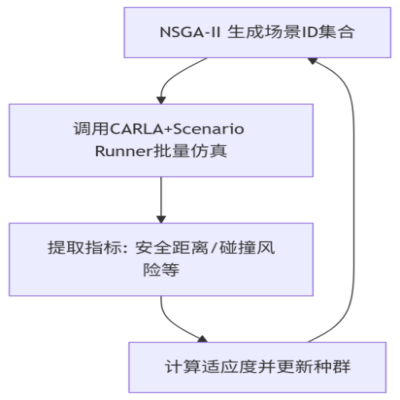
\includegraphics[width=0.8\textwidth]{figure2.png} % 调整宽度为文本宽度的80%
	\caption{NSGA-II算法流程} % 自动编号(如"图1:")
	\label{fig:example} % 用于交叉引用
\end{figure}
\subsection{随机搜索算法设计}
定义参数空间


连续参数:如自车速度(0-120 km/h)、跟车距离(5-50 m)、制动反应时间(0.1-2秒)。

离散参数:如天气条件(晴天、雨天、雾天)、道路类型(高速公路、城市道路、乡村道路)、其他车辆行为(正常行驶、突然变道、急刹车)。

设计评估函数


指标选择:碰撞概率(0-1):通过多次仿真计算碰撞发生频率。

最小安全距离(米):自车与障碍物之间的最小距离。

避让时间(秒):系统从检测到危险到完成避让所需时间。

综合评分公式:危险评分=w1×(1−碰撞概率)+w2×最小安全距离+w3×避让时间危险评分=w1​×(1−碰撞概率)+w2​×最小安全距离+w3​×避让时间(权重 w1,w2,w3w1​,w2​,w3​ 需根据专家经验或数据分析确定)

实现随机采样:

import random

def sample\_parameters(params):

sampled = {}

for key, spec in params.items():

if spec['type'] == 'continuous':

sampled[key] = random.uniform(*spec['range'])

elif spec['type'] == 'discrete':

sampled[key] = random.choice(spec['options'])

return sampled

\newpage
